%
	\section{Heating Mechanisms}\label{sec:heating}
%
        \begin{figure}[!b]
	    	\centering
	    	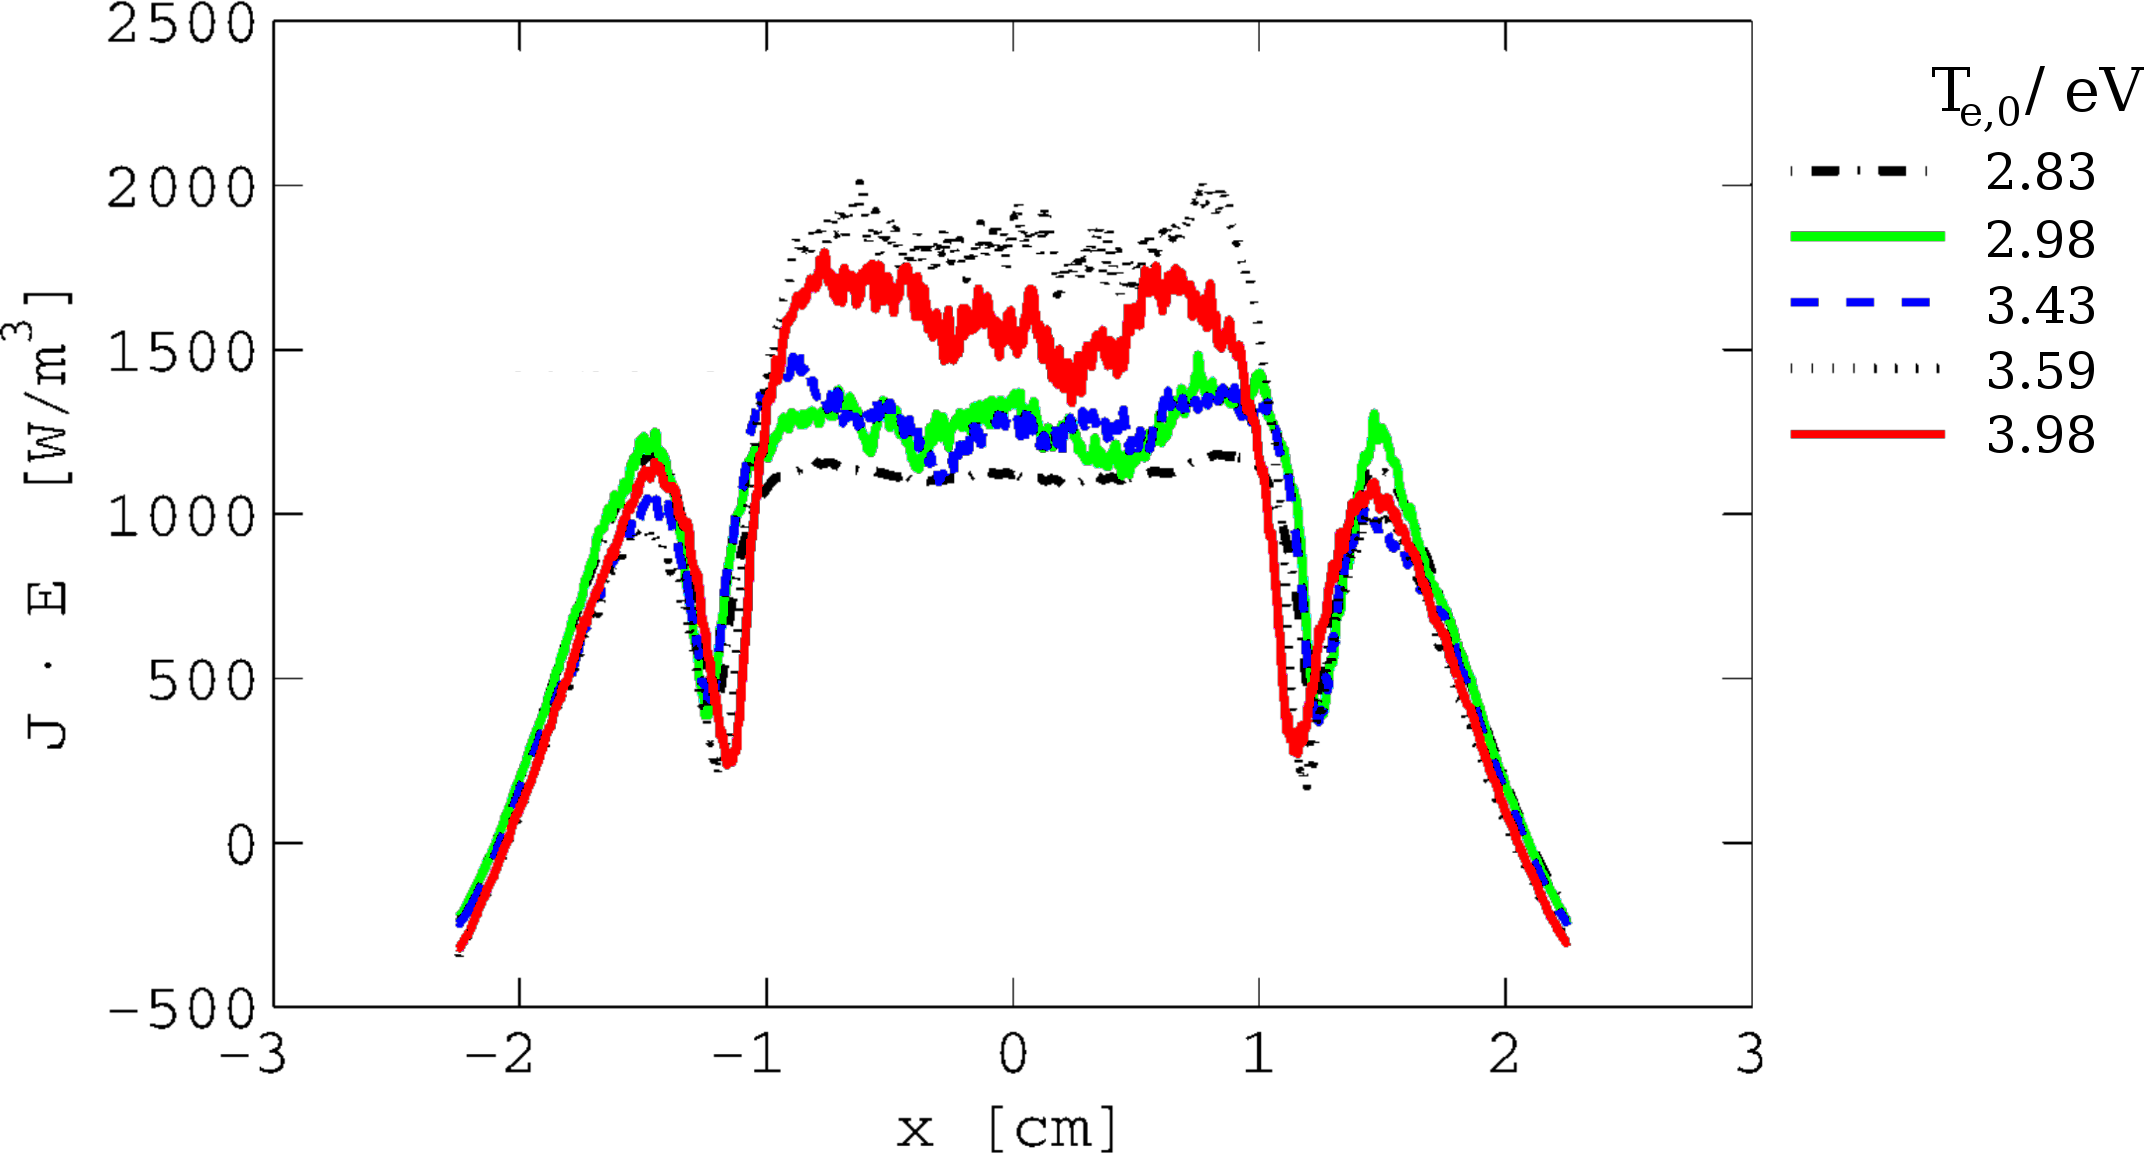
\includegraphics[width=1.0\textwidth]{figures/heatingcomparison.png}
	    	\caption[Electron heating rate in ccrf discharge]{%
	    	Electron heating rate for a ccrf discharge of parallel plates at $\SI{6.7}{\pascal}$ with an electrode gap of $\SI{4.5}{\centi\metre}$ at $\unit[222]{V}$.~\cite{Gudmundsson13}}
	    	\label{fig:heatingcomparison}
	    \end{figure}
%	    
        \paragraph{Ohmic Heating}
	    In a spatially uniform electric field that oscillates harmonically perpendicular to the electrodes, as it is the case in the bulk of a rf plasma, charged particles periodically gain and lose energy in the absence of collisions without any net energy gain~\cite{Schulze09}. This is due to the symmetrical de-/acceleration in the sheaths over one rf cycle. Let us assume the electric field to have no or a negligible component parallel to the electrodes. Hence the mean absorbed power by the charged particles in an oscillating electric field is
%  
	    \begin{align}
	    	\overline{P}\ix{ohm}=\omega\ix{rf}\int_{0}^{T\ix{rf}}\,j\ix{tot}(t)\cdot E(t)\diff t\,,%
	    	\label{equ:meanpowerheat}%
	    	%\\[0.0cm]
	    	%m\ix{e}\frac{\diff v\ix{e}}{\diff t}=-eE(t)-m\ix{e}\nu\ix{n,e}v\ix{e}%
	    	%\label{equ:heatingmotion}
	    \end{align}
%  
	    where $j\ix{tot}$ is the total charge current density. The total mean power dissipated into the charged species through acceleration and neutral gas friction becomes
%  
	    \begin{align}
	    	\overline{P}\ix{ohm}=\frac{|E\ix{0}|^{2}\Re(\sigma\ix{p})}{2}\approx%
	    	\frac{m\ix{e}\nu\ix{n,e}l}{2e^{2}n\ix{e}}j\ix{0}^{2}\,,%
	    	\quad\quad%
	    	\sigma\ix{p}\cong\frac{n\ix{e}e^{2}}{m\ix{e}(\nu\ix{n,e}+\imag\omega\ix{p})}\,.%
%    		\label{equ:ohmicheating}
	    \end{align}
%  
	    Here, $\sigma\ix{p}$ is the plasma conductivity, which yields $j\ix{0}=\sigma\ix{p}E$, and $l$ the bulk length. This demonstrates that power from an spatially uniform, harmonically oscillating electric field can only be transferred via collisions --- the power is zero, if collisions are zero.\\
	    Elastic charged-neutral collisions transfer energy into a direction perpendicular to the field. This component is not lost during the reversal of $E(t)$. Therefore the charged species gain energy during the field oscillation. This mechanism is called \emph{ohmic heating} and takes place mainly in the plasma bulk.\\
         At high pressures, e.g.\@ $>\SI{30}{\pascal}$ ohmic heating is dominant due to the increased neutral gas friction and collisions. In intermediate ranges there is a mode transition to another heating process, which becomes important for lower gas pressures.
%  
	    \paragraph{Stochastic Heating}
	    Heating mechanisms in low pressure ccrf plasmas are of particular importance, because collisions are rare and sheath processes are key to the sustainability of the discharge. Another approach on the heat dissipation in such discharges is connected to the particle acceleration inside the plasma sheath. Here, collisionless energy gain in the sinusoidal modulated space charge in front of a wall is assumed. A `hard wall' approximation (HWA) is made, where the charged particles are considered to collide elastically with the oscillating sheath edge. Heating power is then averaged by reverse and forward energy fluxes into and out of the sheath respectively. This process, though relying on enough randomisation in phase-space inside the bulk, sufficiently creates a net heating of the plasma~\cite{Gozadinos01b,Goedde88}. This is referred to as \emph{stochastic heating}. The parameter $K$ defines the degree of randomisation:
%  
	    \begin{align}
	    	K=\alpha\,\beta\,\frac{U\ix{sb}}{\epsilon E}%
	    	\quad\Leftrightarrow\quad%
	    	E\,<\,m\ix{e}\,\omega^{2}s\ix{0}\,l\,\frac{U\ix{rf}}{U\ix{sb}}\,.%
	    	\label{equ:randomization}
	    \end{align}
%  
           It is derived as a measure of phase-space chaos by electron movement. Chaotic motion occurs in this mapping for $K>1$~\cite{Goedde88}. It decreases with increasing energy, so the system is less stochastic at higher energies. Phase correlations between successive collisions in and with the plasma sheath are reduced at higher energies, and thus decrease stochasticity.\\
	    One can calculate the instantaneous power dissipated into the plasma due to this heating mechanism. Here, using the sheath speed $u\ix{s}$, the electron drift velocity $u\ix{e}$ and the Maxwell electron velocity distribution function $f\ix{v}(v\ix{e},t)$, according Lieberman~\cite{Lieberman88} one can find
%  
	    \begin{align}
	    	P\ix{stoc}(t)=-2m\ix{e}\int_{u\ix{s}}^{\inf}\,u\ix{s}%
	    	{\left(v\ix{e}-u\ix{s}\right)}^{2}\,f\ix{v}(v\ix{e},t)\diff v%
	    	\,\,\approx\,\,%
	    	\frac{m\ix{e}u\ix{e}}{2e^{2}n\ix{e}}j\ix{0}^{2}\,.%
	    	\label{equ:powerdepositheat}
	    \end{align}
%  
         At low pressure, e.g\@ $<\SI{10}{\pascal}$, stochastic heating is the most important energy dissipation process~\cite{Godyak76b,Godyak79}. Figure~\ref{fig:heatingcomparison} the net electron heating rate at given bulk temperatures is shown. Inside the bulk, a plateau can be seen which originates from the stronger ohmic heating in the discharges main volume. Towards the edges of the plasma around +/-\SI{1.5}{\centi\metre} larger peaks in the heating rate build up due to the stochastic heating at the sheath edges. For certain parameters both mechanisms may yield a comparable net heating. Due to significant deviations of the model from the real physics in the HWA~\cite{Gudmundsson13,Lieberman88}, ohmic heating might be considered a more reliable assumption as the plasmas main heat generation process.
%
%		\begin{align}
%			\tau\ix{n}\approx\frac{2\alpha(\mu\ix{n}-\beta%
%				\cos\varphi\ix{n})}{1+\alpha\beta\cos\varphi\ix{n}}\,,%
%			\quad\quad%
%			\mu\ix{n+1}=-\mu+\frac{2(\mu\ix{n}-%
%           \beta\sin\varphi\ix{n})}{1+\alpha\beta\cos\varphi\ix{n}}%
%			\label{equ:transitandvelocityheating}
%		\end{align}
%
%		In \emph{hamiltonian mappings}, those two variables are not canonically conjugate, hence insufficient for checking conserved quantities. One has to keep that in mind when evaluating the HWA approximation. The change in velocity in one pass through the sheath becomes the impulse approximation of the \emph{Fermi acceleration}m which is written as:
%
%		\begin{align}
%			\Delta v=v\ix{n+1}-v\ix{n}=-2\,\omega\,%
%			s\ix{0}\frac{U\ix{rf}}{U\ix{sb}}\,\sin\varphi\ix{n}\,.%
%			\label{equ:deltavheating}
%		\end{align}
%
%		The results on the right-hand-side yields not net heating if averaged over one rf cycle, if the current used would be conserved in a manner the HWA is predicting it, or the electron drift velocity does not satisfy the Maxwellian distribution function. Hence there have to be deviations from the proposed theory of stochastical heating. This would be e.g.\@ ab initio information about the EEDF, unconsidered transit time effects of the sheath electric field and neglected particle losses and current conservation.\\
%		There are more theoretical approaches on the heating in low-pressure, low-temperature rf plasma. For example, Surendra et al~\cite{Surendra93} put forth the idea that the compression and decompression of the electron density volume between opposing plasma sheaths generates heat inside the bulk, which is responsible for the observed heating.\\
%		The electron heating profile is shown in~\autoref{fig:heatingcomparison}, with peaks near the sheath edges due to stochastic heating while the main plateau in the bulk is a result of the dominantly strong ohmic heating with slow electrons and neutral gas friction.\\
%       Consider the sheaths electric field as constant, $E=U\ix{sb}/s\ix{0}$, the bulks expansion to be $l$ and the sheaths thickness $d$ being modulated cosinusoidal. The equation of motion for an electron in the sheath is taken from above, cancelling out the part of ohmic neutral gas heating.
%
%		\begin{align}
%			d(t)\approx s\ix{0}\left(1+\frac{U\ix{rf}}{U\ix{sb}}\cos\left(\omega t\right)\right)%
%			\label{equ:sheaththickness}
%		\end{align}
%
%	    The \autoref{equ:heatingmotion} is introduced to be dimensionless with the substitution of the corresponding parameters: $\alpha=m\ix{e}\omega^{2}s\ix{0}^{2}/(eU\ix{sb})$, $\beta=U\ix{rf}/U\ix{sb}$ and $\epsilon=s\ix{0}/l\,$. Integration yields the velocity $\mu(\tau)$ of an electron as it moves through the sheath. The transit time $\tau$ is considered for one pass through the sheath of the particle. It can be used to calculate the change in velocity experienced by the electron on each bounce between this oscillating and a fixed wall --- this would be the lowest order \emph{fermi acceleration}. Assuming there are two distinct moments and positions, where the particle enters (index $n$) and re-enters (index $n+1$) the sheath, this gives, using $\varphi\ix{n}$ the phase of the sheath, for the transit time and velocity~\cite{Goedde88}
%		
%		\begin{figure}[t!]
%			\centering
%  		\begin{longtable}{lccccr}
%				\toprule%
%					Case & $\Phi\ix{0}$ & $n\ix{e,0}$/$\unit{m^{-3}}$ %
%					& $n\ix{i-,0}$/$\unit{m^{-3}}$ & $n\ix{i+,0}$/$\unit{m^{-3}}$ %
%					&	$T\ix{e,0}$/$\unit{eV}$ \\%
%		    \toprule\midrule\endhead%
%				1 & 101.30 & \SI{2.43e14} & \SI{1.17e16} & \SI{1.20e16} & 2.83 \\ \midrule%
%				2 & 101.25 & \SI{2.29e14} & \SI{1.21e16} & \SI{1.23e16} & 2.98 \\ \midrule%
%				3 & 101.75 & \SI{2.18e14} & \SI{1.19e16} & \SI{1.20e16} & 2.98 \\ \midrule%
%				4 & 103.11 & \SI{1.55e14} & \SI{1.75e16} & \SI{1.78e16} & 3.59 \\ \midrule%
%				5 & 102.55 & \SI{1.65e14} & \SI{1.70e16} & \SI{1.71e16} & 3.43 \\ \midrule%
%    	\bottomrule%
%			\caption{%
%				Selected plasma parameters for the used cases in~\autoref{fig:heatingcomparison} %
%				at the center of the discharge.~\cite{Gudmundsson13}}\label{tab:comparisonheating}
%			\end{longtable}
%		\end{figure}